% Created 2021-03-01 Mon 19:28
% Intended LaTeX compiler: pdflatex
\documentclass[11pt]{article}
\usepackage[utf8]{inputenc}
\usepackage[T1]{fontenc}
\usepackage{graphicx}
\usepackage{grffile}
\usepackage{longtable}
\usepackage{wrapfig}
\usepackage{rotating}
\usepackage[normalem]{ulem}
\usepackage{amsmath}
\usepackage{textcomp}
\usepackage{amssymb}
\usepackage{capt-of}
\usepackage{hyperref}
\author{Leandro Lupori Vanderson Martins do Rosario Edson Borin}
\date{\today}
\title{Towards a High-Performance RISC-V Emulator\\\medskip
\large Dążąc do wydajnego emulatora RISC-V}
\hypersetup{
 pdfauthor={Leandro Lupori Vanderson Martins do Rosario Edson Borin},
 pdftitle={Towards a High-Performance RISC-V Emulator},
 pdfkeywords={},
 pdfsubject={},
 pdfcreator={Emacs 27.1 (Org mode 9.3)}, 
 pdflang={English}}
\begin{document}

\maketitle
\tableofcontents \clearpage\url{https://ieeexplore.ieee.org/document/8748908}

\section{Dążąc do wydajnego emulatora RISC-V}
\label{sec:orgd88d9a1}
RISC-V jest otwartą architekturą procesora która zwróciła uwage całego swiata poprzez swój szybki rozwój i adaptacje. Jest ona juz wspierana przez GCC, Clang, i Linux. Ponadto niedawno
pojawiło się wiele emulatorów i symulatorów RISC-V, niestety żaden z nich nie jest wystarczająco wydajny. Zazwyczaj, najczęściej stosowaną i najszybszą metodą implementacji takich emulatorów jest DBT - dynamiczna translacja maszynowa (\emph{z ang.Dynamic Binary Translation}), która wymaga dobrej jakości translacji by uzyskać wysoką wydajność. W tej pracy zbadamy czy wysokiej jakości translacja kodu maszynowego RISC-V jest możliwa. W tym celu użylyliśmy SBT - statycznej translacji binarnej (\emph{z ang. Static Binary Translation}) by sprawdzić jakość jaka może być uzyskana przy tłumaczeniu RISC-V na x86 i ARM. Nasze wyniki experymentalne pokazują że nasz SBT potrafi stworzyć wysokiej jakości kod, otrzymując tylko 12\%/35\% nizsza wydajnośc w porównaniu do kompilowanego kodu x86/ARM. Jest to lepszy wynik niż inne bardziej znane dynamiczne translatory RISC-V takie jak RV8 i QEMU. Ponieważ dynamiczna translacja jest silnie związana z jakościa translacji, nasz statyczny translator pokazuje że istnieją możliwości stworzenia bardziej wydajnych dynamicznych translatorów RISC-V niż obecnie istniejące
\section{Spis treści}
\label{sec:org98042da}
\begin{enumerate}
\item Wprowadzenie
\item Translacja kodu maszynowego i Wyzwania
\item RISC-V
\item Powiązane prace
\item Dynamiczna translacja RISC-V
\begin{enumerate}
\item niezlinkowany kod maszynowy jako wejscie
\item mapowanie rejestrów
\end{enumerate}
\item Środowisko eksperymentalne
\begin{enumerate}
\item Metodologia pomiarowa
\item GCC vs Clang i opcje operacji zmiennoprzecinkowych
\item Konfiguracja RISC-V
\end{enumerate}
\item Wyniki eksperymentów
\begin{enumerate}
\item GCC vs Clang
\item RISC-V vs openISA
\item Nasz SBT vs dostępne DBTv
\end{enumerate}
\item Wnioski
\end{enumerate}
\section{Przedstawienie wyników}
\label{sec:orgd8e2e17}
Wyniki sa przedstawione w postaci tabeli porównujących programy kompilowane na x86/ARM do programów statycznie przetłumaczonych za pomocą nowego SBT oraz istniejących translatorów (RV8 i QEMU). Porównywane są różne ustawienia kompilatorów i ich wpływ na wyniki oraz porównanie do translacji openISA
\begin{center}
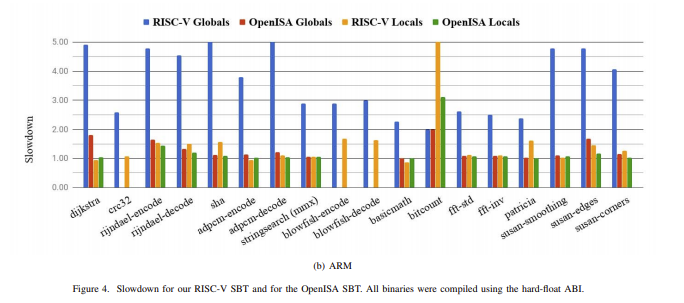
\includegraphics[width=.9\linewidth]{./figure4.png}
\end{center}
\begin{center}
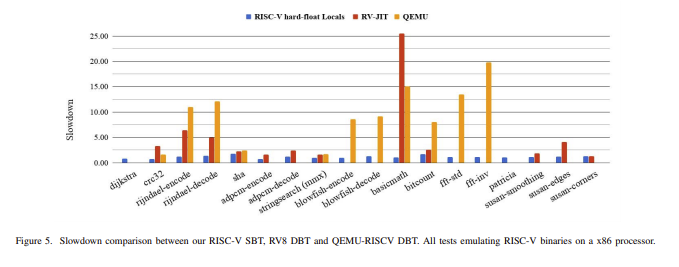
\includegraphics[width=.9\linewidth]{./figure5.png}
\end{center}
\section{Interpretacja wyników}
\label{sec:orga1773f9}
Po porównaniu stworzonego silnika translacji statycznej stwierdzili że zbudowanie wydajnego emulatora RISC-V na sprzęcie dostępnym dzisiaj (W wiekszosci x86 i ARM). Oczekują rownież używanie tej otwartej architektury jako IR (kod binarny gotowy do translacji wynikowej)
\end{document}
